\section{Background}
%%%%%%%%%%%%%%%%%%%%%%%%%%%%%%%%%%%%%%%%%%%%%%%%%%%%%%%%%%%%%%%%%%%%%%%%%%%%%%%%%%%%%%%%%%%%%%%%%%%%
% The Flow Based Model
%%%%%%%%%%%%%%%%%%%%%%%%%%%%%%%%%%%%%%%%%%%%%%%%%%%%%%%%%%%%%%%%%%%%%%%%%%%%%%%%%%%%%%%%%%%%%%%%%%%%
\subsection{Flow Based Model}

Flow-based models define an invertible transformation between a simple prior distribution and a target data distribution.

Let $x$ denote a random variable following a simple prior distribution, such as the standard Gaussian, and let $y$ denote a variable following the target distribution. Then there exists a mapping $f: \mathbb{R}^d \to \mathbb{R}^d$ such that $y = f(x)$.
By the change of variable formula, the probability density funciton of $x$ and $y$ relates with:

\begin{equation}
  p_Y(y) = p_X(x) \frac{\partial x}{\partial y},
\end{equation}
%
where $\dfrac{\partial x}{\partial y}$ is the Jacobian matrix of the inverse transformation $f^{-1}$.

With this formula, we can learn the mapping function $f$ directly, and this explicit relationship makes the flow-based model interpretable. However, computing the Jacobian determinant is usually computational expensive, and this constrains the model design.

%%%%%%%%%%%%%%%%%%%%%%%%%%%%%%%%%%%%%%%%%%%%%%%%%%%%%%%%%%%%%%%%%%%%%%%%%%%%%%%%%%%%%%%%%%%%%%%%%%%%
% Flow Matching
%%%%%%%%%%%%%%%%%%%%%%%%%%%%%%%%%%%%%%%%%%%%%%%%%%%%%%%%%%%%%%%%%%%%%%%%%%%%%%%%%%%%%%%%%%%%%%%%%%%%
\subsection{Flow Matching}

%%%%%%%%%%%%%%%%%%%%%%%%%%%%%%%%%%%%%%%%%%%%%%%%%%%%
% Continuity Equation and Velocity Field
%%%%%%%%%%%%%%%%%%%%%%%%%%%%%%%%%%%%%%%%%%%%%%%%%%%%
\subsubsection{Continuity Equation and Velocity Field}

The continuity equation describes how a density evloves with a velocity field. Let $v(x, t)$ and $\rho(x, t)$ denote the velocity field and the density of a substance at position $x$ and time $t$. The continuity equation is given by:
%
\begin{equation}
  \frac{\partial \rho(x, t)}{\partial t} + \nabla_x \cdot \left( \rho(x, t) v(x, t) \right) = 0.
\end{equation}

It states that, for any infinitesimal volume, the change of the density inside the volume equals the net flux across the boundary. This local balance, under some reasonable assumptions like the convergence of the global density, implies the global conservation of the substance. In our case, the ``total substance'' corresponds to the probability mass, and $\rho (x, t)$ represents the probability density. As a distribution evloves from a prior to the target data distribution, the continuity equation motivates the use of a velocity field to describe this evolution.

Let $p_\text{prior}$ and $p_\text{target}$ denote the prior and the target distribution, and let $x_0 \sim p_\text{prior}$ and $x_1 \sim p_\text{target}$. Suppose the distribution evolves from $t = 0$ to $t = 1$ with intermediate distribution $p_t$ and $x_t \sim p_t$, we defined the velocity field $v(x_t, t)$ as:
%
\begin{equation}\label{ode}
  v(x_t, t) \triangleq \frac{d x_t}{d t}.
\end{equation}
%
Given $v(x_t, t)$, a sample from $p_t$ can be obtained by:
%
\begin{equation}
  x_t - x_0 = \int_0^t v(x_\tau, \tau) \, d \tau.
\end{equation}
%
In particular, selecting $t = 1$ produces a sample from $p_\text{target}$.

\begin{figure}[t]
  \vspace{-3em}
  \centering
  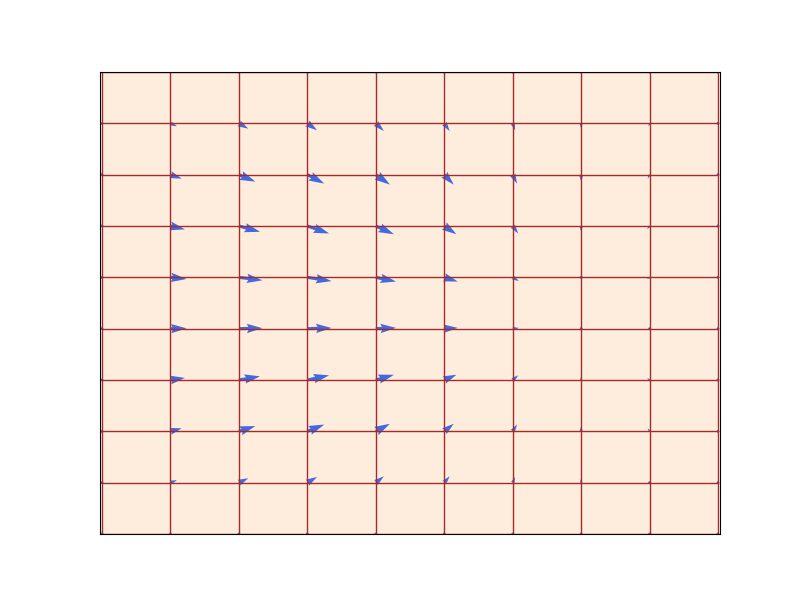
\includegraphics[width=0.32\textwidth]{figures/flow_1.png}%
  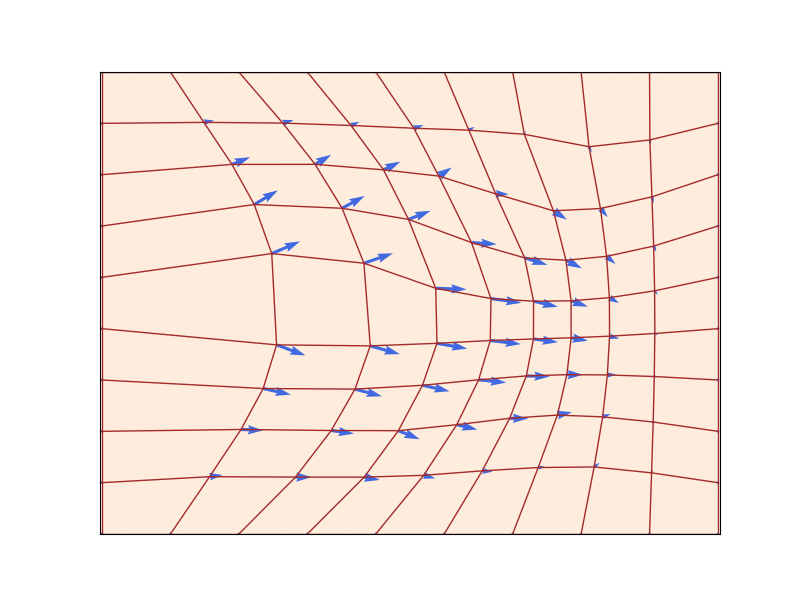
\includegraphics[width=0.32\textwidth]{figures/flow_2.png}%
  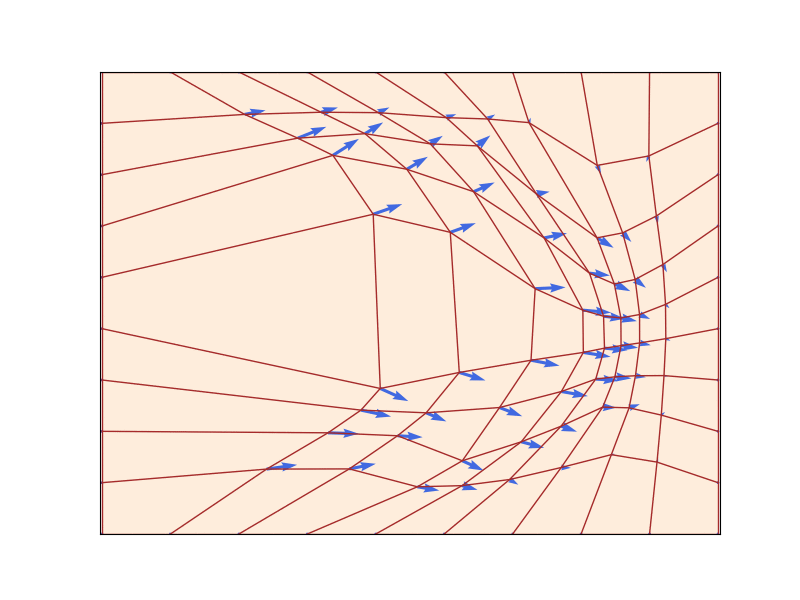
\includegraphics[width=0.32\textwidth]{figures/flow_3.png}%
  \vspace{-1em}
  \caption{Illustration of flows. Here, the evolution of the density is defined by a velocity field $v: \mathbb{R}^d \to \mathbb{R}^d$ (blue arrows) specifying its instantaneous movements at all locations (here $d = 2$). Figure from~\cite{flow}.}
\end{figure}

%%%%%%%%%%%%%%%%%%%%%%%%%%%%%%%%%%%%%%%%%%%%%%%%%%%%
% Probability Path and Training Target
%%%%%%%%%%%%%%%%%%%%%%%%%%%%%%%%%%%%%%%%%%%%%%%%%%%%
\subsubsection{Probability Path and the Training Target}

A deterministic trajectory from $p_\text{prior}$ to $p_\text{target}$ is called a probability path or marginal probability path. This evolution is driven by the marginal velocity field $v(x_t, t)$. However, directly obtaining $v(x_t, t)$ is generally difficult. Flow Matching constructs an equivalent velocity $v^\text{tgt}(x_t, t)$ with the weighted average.

Consider sampling $z$ from $p_\text{target}$ and defining a conditional probability path from $p_\text{prior}$ to $\delta_z$ with conditional distribution $p_t(\cdot \mid z)$:
%
\begin{equation}
x_t = (1 - t) x_0 + t z.
\end{equation}
%
The marginal distribution is then given by the total probability throrem:
%
\begin{equation*}
p_t(x_t) = \int p_t(x_t \mid z) p_\text{target}(z) \, dz.
\end{equation*}
%
The corresponding conditional velocity field is:
%
\begin{equation}\label{ode_cond}
  v(x_t, t \mid z) \triangleq \frac{d x_t}{d t} = z - x_0.
\end{equation}
%
The marginal velocity, which serves as the training target, is constructed by taking the expectation of the conditional velocity under the weights of $z$:
%
\begin{align}
  v^\text{tgt}(x_t, t) &\triangleq \int v(x_t, t \mid z) p_t(z \mid x_t) \, d z \nonumber \\
  &= \int v(x_t, t \mid z) \frac{p_t(x_t \mid z) p_\text{target}(z)}{p_t(x_t)} \, dz.
\end{align}
%
The validity of this construction with respect to $v^\text{tgt} (x_t, t)$ is discussed in Appendix~\ref{app:continuity}.

\begin{figure}[t]
  \vspace{-3em}
  \centering
  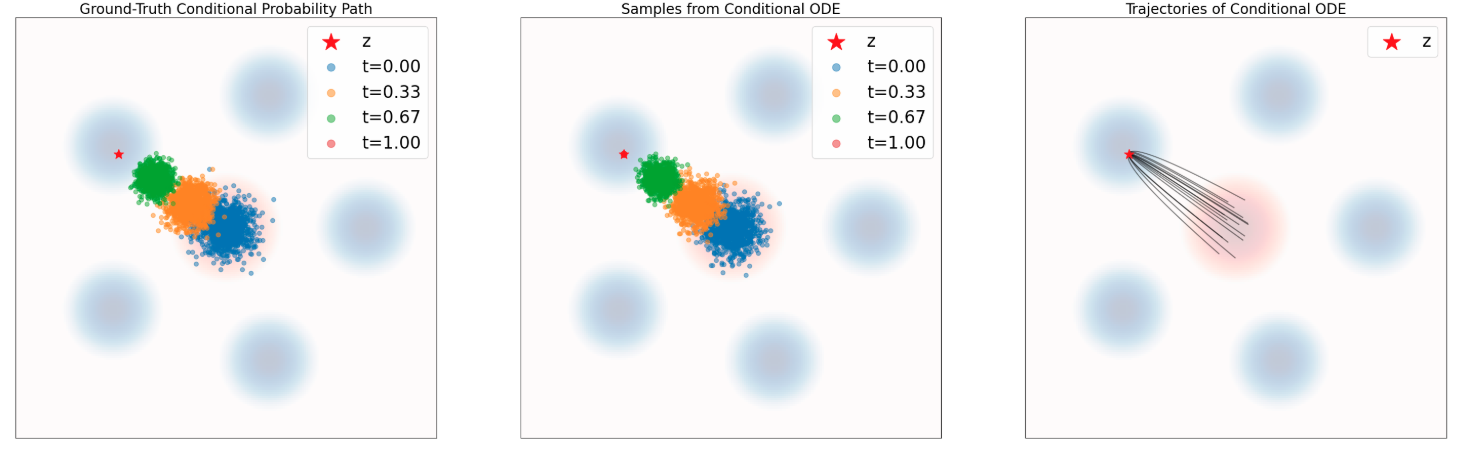
\includegraphics[width=\textwidth]{figures/conditional_probability_path.png}
  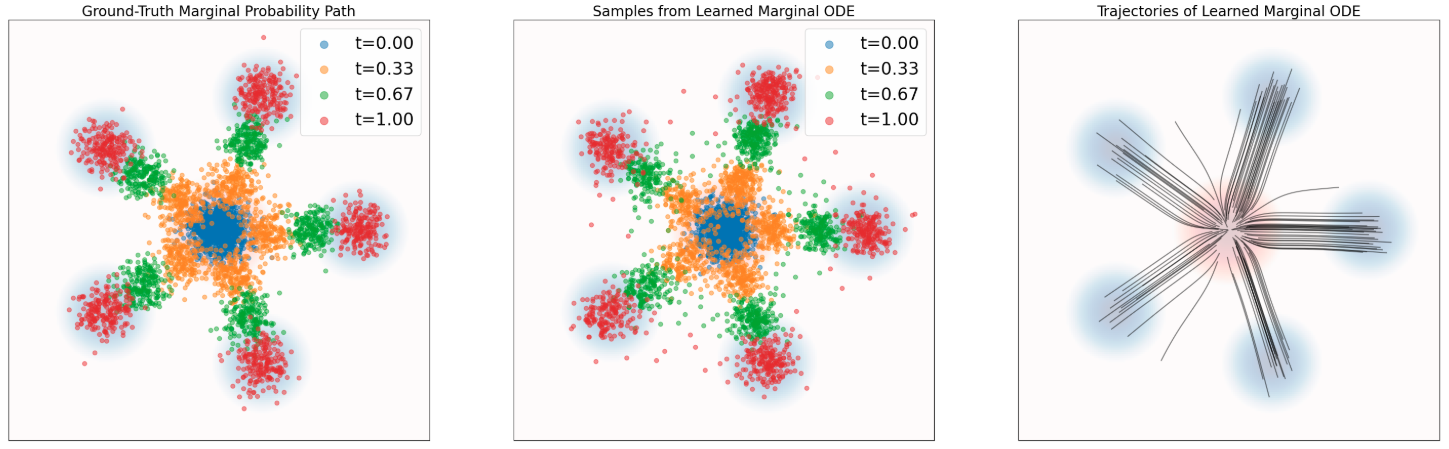
\includegraphics[width=\textwidth]{figures/marginal_probability_path.png}
  \vspace{-1em}
  \caption{Illustration of conditional and marginal probability path. Target distribution $p_\text{target}$ in blue background. Gaussian prior distribution $p_\text{prior}$ in red background. Top row: Conditional probability path. Left: Ground truth samples from $p_t(\cdot \mid z)$. Middile: ODE samples over times. Right: Trajectories by simulating ODE in Equation~\eqref{ode_cond}. Bottom row: Simulating a marginal probability path. Left: Ground truth samples from $p_t$. Middle: ODE samples over times. Right:  Trajectories by simulating ODE in Equation~\eqref{ode}. As one can see, the conditional vector field follows the conditional probability path and the marginal vector field follows the marginal probability path. Figure from~\cite{mit}.}
  \vspace{2em}
\end{figure}

%%%%%%%%%%%%%%%%%%%%%%%%%%%%%%%%%%%%%%%%%%%%%%%%%%%%
% Train the Model
%%%%%%%%%%%%%%%%%%%%%%%%%%%%%%%%%%%%%%%%%%%%%%%%%%%%
\subsubsection{Train the Model}\label{train_model}

Our generative model is trained by fitting a neural network $v^\theta(x_t, t)$ to approximate the target velocity field $v^\text{tgt}(x_t, t)$. A natural choice is the mean squared error (MSE) loss:
%
\begin{equation}
  \mathcal{L_\text{FM}} (\theta) = \mathbb{E}_{t, x_t \sim p_t} \left[ \left\| v^\theta (x_t, t) - v^\text{tgt} (x_t, t) \right\|_2^2 \right]
\end{equation}
%
However, there is no closed-form for $v^\text{tgt}(x_t, t)$, and what we have access to is only samples from $p_\text{target}$ and $p_\text{prior}$. We now show that, under the MSE loss, one may equivalently replace $v^\text{tgt} (x_t, t)$ with the conditional velocity field $v(x_t, t \mid z)$:
%
\begin{equation}
  \mathcal{L_{\text{CFM}}} (\theta) = \mathbb{E}_{t, z \sim p_\text{target}, x_t \sim p_t(\cdot \mid z)} \left[ \left\| v^\theta (x_t, t) - v^\text{tgt} (x_t, t \mid z) \right\|_2^2 \right],
\end{equation}
%
and the two objectives share the same gradients:
\begin{equation}
  \nabla_\theta \mathcal{L_{\text{CFM}}} (\theta) = \nabla_\theta \mathcal{L_{\text{FM}}} (\theta).
\end{equation}

\paragraph{Proof.}
Expanding the square in $\mathcal{L_\text{FM}}$ and $\mathcal{L_\text{CFM}}$, we obtain
\begin{align*}
   \mathcal{L_{\text{FM}}} (\theta) &=  \mathbb{E}_{t, x_t \sim p_t} \left[ \left\| v^\theta (x_t, t) \right\|_2^2 \right] - 2 \mathbb{E}_{t, x_t \sim p_t} \left[ \left\| {v^\theta (x_t, t)}^\top v^\text{tgt} (x_t, t)\right\|_2^2 \right] + \mathbb{E}_{t, x_t \sim p_t} \left[ \left\| v^\text{tgt} (x_t, t) \right\|_2^2 \right] \\
    \mathcal{L_{\text{CFM}}} (\theta) &= \mathbb{E}_{t, z \sim p_\text{target}, x_t \sim p_t(\cdot \mid z)} \left[ \left\| v^\theta (x_t, t) \right\|_2^2 \right] - 2  \mathbb{E}_{t, z \sim p_\text{target}, x_t \sim p_t(\cdot \mid z)} \left[ {v^\theta (x_t, t)}^\top v^\text{tgt} (x_t, t \mid z) \right] \\
    &\quad + \mathbb{E}_{t, z \sim p_\text{target}, x_t \sim p_t(\cdot \mid z)} \left[ \left\| v^\text{tgt} (x_t, t \mid z) \right\|_2^2 \right]
\end{align*}
%
For the cross term, we compute
%
\begin{align*}
\mathbb{E}_{t, x_t \sim p_t} \left[ {v^\theta(x_t, t)}^\top v^\text{tgt}(x_t, t) \right] &= \iint {v^\theta(x_t, t)}^\top v^\text{tgt}(x_t, t) p_t(x_t) \, dt \, dx_t \\
&= \iint {v^\theta(x_t, t)}^\top \left( \int v(x_t, t \mid z) \frac{p_t(x_t \mid z) p_\text{target}(z)}{p_t(x_t)} \, dz \right) p_t(x_t) \, dt \, dx_t \\
&= \iiint {v^\theta(x_t, t)}^\top v(x_t, t \mid z) p_t(x_t \mid z) p_\text{target}(z) \, dz \, dt \, dx_t \\
&= \mathbb{E}_{t, z \sim p_\text{target}, x_t \sim p_t(\cdot \mid z)} \left[ {v^\theta(x_t, t)}^\top v(x_t, t \mid z) \right]
\end{align*}

The expectation of $v^\theta(x_t, t)$ are identical under two different measures, thus $\mathcal{L_{\text{FM}}}$ and $\mathcal{L_{\text{CFM}}}$ differ only in terms independent of $\theta$. Since such terms vanish under gradient, $\nabla_\theta \mathcal{L_{\text{CFM}}} (\theta) = \nabla_\theta \mathcal{L_{\text{FM}}} (\theta)$.

More generally, for any error function that is linear in $v^\text{tgt}(x_t, t)$, one may substitute $v^\text{tgt}(x_t, t)$ with $v(x_t, t \mid z)$ without affecting the optimization (see Appendix~\ref{app:linear_func}).
